\subsection{IFIT2B}
IFIT2B -> stuff detected by anti-IFIT2 antibody B

Everything stated in this subchapter is only attributable to the staining seen with IFIT2 antibody B
\subsubsection{Nascent Human and Monkey IFIT2 in a Simplified System of pseudo-IBs} \label{Nascent Human and Monkey IFIT2 in a Simplified System of pseudo-IBs}
\myparagraph{Nascent Human and Monkey IFIT2 in pIBs}
\mysubparagraph{i2b vero hnhp}
Cell Line: VERO \newline
Treatment: hNhP \newline
Detecting magenta: endogenous monkey IFIT2 \newline
Detecting cyan: human pIB \newline

Nascent monkey IFIT2 is completely excluded from the human RSV pseudo-IBs and the pIB filamentous network.

\begin{figure}
    \centering
    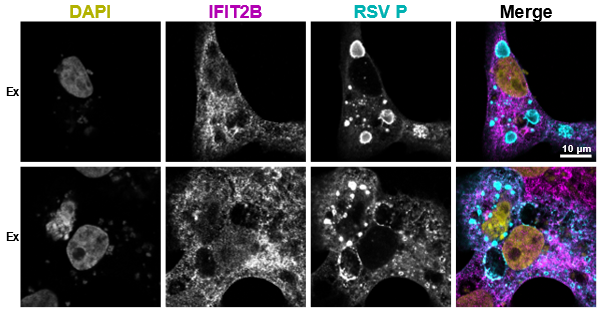
\includegraphics[width=1\linewidth]{09. Chapter 4//Figs//02. I2B/01. i2b vero hnhp.png}
    \caption[i2b vero hnhp]{i2b vero hnhp}
    \label{i2b vero hnhp}
\end{figure}

\myparagraph{Exogenous Human and Bovine IFIT2 in pBs}
\mysubparagraph{i2b vero hi2 + hnhp}
Cell Line: VERO \newline
Treatment: hNhP + hIFIT2-FLAG \newline
Detecting magenta: endogenous monkey IFIT2 + exogenous human IFIT2 \newline
Detecting cyan: human pIB \newline

Monkey cells transfected with human RSV N and P, along with human IFIT2-FLAG show concentration within the pIB structures but show exclusion from the pIB filamentous network (or partial colocalsiation?). This suggest that the IFIT2B antibody can indeed detect IFIT2 but the overexpressed IFIT2 observed between the inclusion and the one interacting with the filamentous network is somehow different (epitope masking?).

\begin{figure}
    \centering
    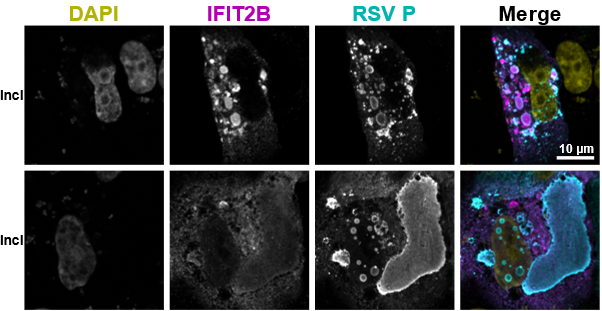
\includegraphics[width=1\linewidth]{09. Chapter 4//Figs//02. I2B/02. i2b vero i2 hnhp.png}
    \caption[i2b vero hi2 + hnhp]{i2b vero hi2 + hnhp}
    \label{i2b vero hi2 + hnhp}
\end{figure}

\subsubsection{Nascent Human and Bovine IFIT2B Localisation During h/bRSV Infection} \label{Nascent Human and Bovine IFIT2A Localisation During h/bRSV Infection}
\myparagraph{hIFIT2B localisation during hRSV Infection}
\mysubparagraph{i2b a549 hrsv}
Cell Line: A549 \newline
Treatment: hRSV \newline
Detecting magenta: endogenous human IFIT2  \newline
Detecting cyan: human IB \newline

Endogenous human IFIT2 is either partially excluded (top panel; decrease of intra IB signal compared to cytoplasmic signal) or completely excluded (bottom panel) from the human IB structure.

\begin{figure}
    \centering
    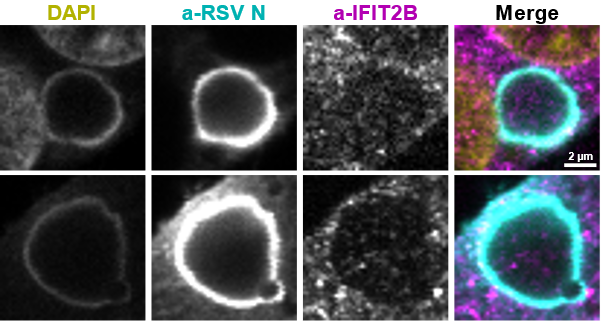
\includegraphics[width=1\linewidth]{09. Chapter 4//Figs//02. I2B/03. i2b a549 hrsv n.png}
    \caption[i2b a549 hrsv n]{i2b a549 hrsv n}
    \label{i2b a549 hrsv n}
\end{figure}

Cell Line: A549 \newline
Treatment: hRSV \newline
Detecting magenta: endogenous human IFIT2  \newline
Detecting cyan: human IB  \newline

We observe similar pattern of staining to what was observed with N stained human IBs. IFIT2 signal is either partially or totally excluded from the IB structure.

\begin{figure}
    \centering
    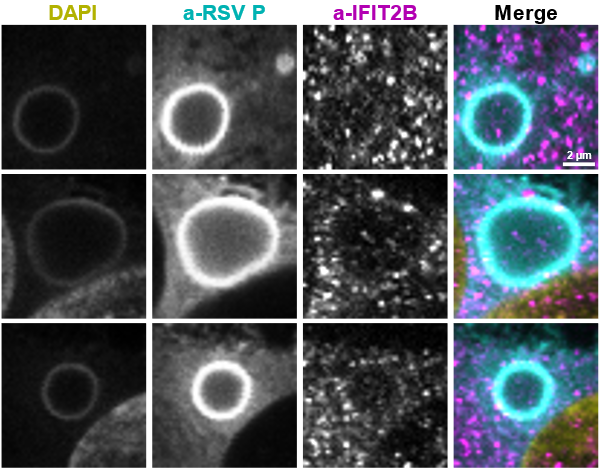
\includegraphics[width=1\linewidth]{09. Chapter 4//Figs//02. I2B/04. i2b a549 hrsv p.png}
    \caption[i2b a549 hrsv p]{i2b a549 hrsv p}
    \label{i2b a549 hrsv p}
\end{figure}

Cell Line: A549 \newline
Treatment: hRSV \newline
Detecting magenta: endogenous human IFIT2  \newline
Detecting cyan: human IB \newline

Endogenous human IFIT2 seems to be excluded from hRSV IBs.

\begin{figure}
    \centering
    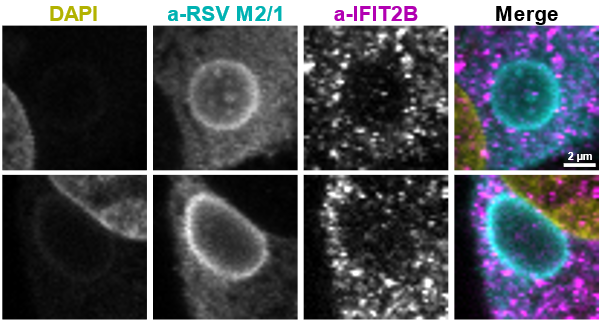
\includegraphics[width=1\linewidth]{09. Chapter 4//Figs//02. I2B/05. i2b a549 hrsv m21.png}
    \caption[i2b a549 hrsv m21]{i2b a549 hrsv m21}
    \label{i2b a549 hrsv m21}
\end{figure}

\mysubparagraph{i2b beas2b hrsv}
some text

\begin{figure}
    \centering
    
\includegraphics[width=0.5\linewidth]{09. Chapter 4//Figs//02. I2B/00. placeholder.png}
    \caption[i2b beas2b hrsv]{i2b beas2b hrsv}
    \label{i2b beas2b hrsv}
\end{figure}

\myparagraph{hIFIT2B localisation during bRSV Infection}
\mysubparagraph{i2b mdbk brsv}
Cell Line: MDBK \newline
Treatment: bRSV + bIFNa \newline
Detecting magenta: endogenous bovine IFIT2  \newline
Detecting cyan: bovine IB \newline

Endogenous bovine IFIT2 localisation with respect to the bovine inclusion bodies shows a few different phenotypes. We see partial exclusion (to panel; signal still present in the middle of the IB structure), exclusion from IB ring and the inner IB edge (middle panel; highlighted with arrow) with IBAG-like concentrations inside the structure; and diffusion through the IB structure (bottom panel). These phenotypes are similar to what is observed during RSV infection of human but especially bovine IFIT3 and IFIT5.

\begin{figure}
    \centering
    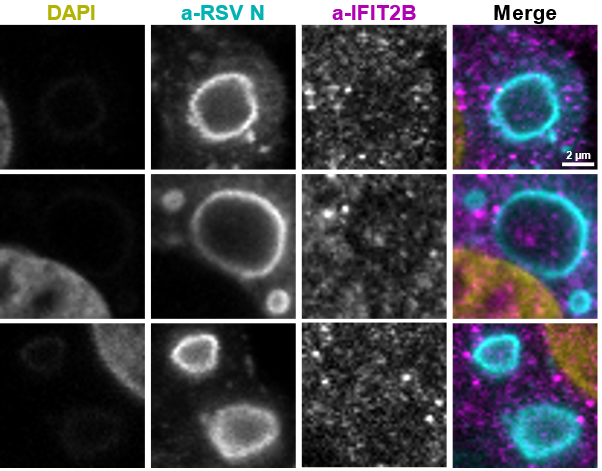
\includegraphics[width=1\linewidth]{09. Chapter 4//Figs//02. I2B/06. i2b mdbk brsv.png}
    \caption[i2b mdbk brsv]{i2b mdbk brsv}
    \label{i2b mdbk brsv}
\end{figure}

\subsection{Summary} \label{Summary}
Endogenous monkey IFIT2 is excluded from human pIB and the pIB associated filamentous network. Overexpressed human IFIT2-FLAG is detected by the antibody and shows inclusions inside the human pIB structures, which is consistent to data from IFIT2A staining and FLAG staining of IFIT2-FLAG overexpressed samples. Interestingly, IFIT2B antibody shows exclusion from the pIB filamentous network, which was colocalised by IFIT2A and FLAG antibodies. Nascent human IFIT2 shows full or partial exclusion from human IBs during human RSV infection. Nascent bovine IFIT2 during bRSV infections shows 3 different phenotypes. We observed partial exclusion; exclusion from the IB ring and inner edge with IBAG-like inclusions; and diffusion through the IB structure. This staining is similar to what is observed with bovine IFIT3 and IFIT5 during bRSV infection.